\documentclass{article}
\usepackage[utf8]{inputenc}
\usepackage[margin=2.5cm]{geometry}
\usepackage{graphicx}
\usepackage{subfigure}
\usepackage{varioref}

\providecommand{\keywords}[1]{
    \small
    \textbf{Keywords: } #1
}

\title{Intelligent Linguistic System for the Grammar of the Romanian Language}
\author{Ioan Florin Cătălin Nițu, Traian Eugen Rebedea\\
University Politehnica of Bucharest}
\date{June - July 2020}

\bibliographystyle{apalike}

\begin{document}
    
    \maketitle
    
    \begin{abstract}
        
        The field of natural language processing is not as strongly developed for the Romanian language as it is for others, as is the English language. Writing texts correctly has always been a necessity, and the development of tools that will be useful in this need is critical. The proposed correction system receives a sentence with grammatical errors and corrects it, using state-of-the-art technologies to perform this operation such as attention-based neural models like Encoder-Decoder Transformers. These are a cornerstone in the development of intelligent tools for processing – translating, summarizing, or proofreading – texts and are the foundation for this project. The paper uses RONACC, the first corpus for grammatical corrections in Romanian for modeling, training, testing, and validating the project. Using a very large data set with over a million learning examples, an average BLEU score of 45.29 points was obtained, in a rather short training time (only two hours for five epochs) executed on several GPUs. However, even a small data set of only fifty thousand examples with as many as one hundred epochs achieves an average BLEU score of 33.29 points in three hours.  \cite{nitu2020intelligent}
        
        \keywords{Romanian language, grammar, transformers, attention, positional encoding}
        
    \end{abstract}
    
    \section{Introduction}
        
        Correcting texts and natural language, in general, is often encountered in computer science, artificial intelligence, and machine learning. The study of natural language processing has brought technologies, models, and products that can competitively address this issue.
        
    \section{Related Word}
        
        This paper uses Python and TensorFlow to implement a Transformer-based solution proposed in the article Attention Is All You Need \cite{vaswani2017attention}. Attention mechanisms have become an integral part of persuasive sequence models and reasoning models in different tasks, allowing dependency modeling without considering their distance in input or output sequences \cite{bahdanau2014neural}. In most cases, such attention mechanisms are used in conjunction with a recurring network. Transformers are introduced as a model architecture that avoids recurrences and relies on an attention mechanism to attract global dependencies between input and output. The transformer allows a significantly higher parallelization and can reach a new stage in terms of the quality of translation or correction of texts after training \cite{vaswani2017attention}.
        
    \section{Method}
        
        The data set used to train, validate and test the model is the RONACC corpus. The data set consists of pairs of lines of correct and wrong sentences. Training is done in several epochs. From time to time, after some epochs, a checkpoint is made to save the training done. The transformer is an auto-regressive model \cite{graves2013generating}: it makes predictions one at a time and uses its output so far to decide what to do next \cite{tensorflow2019transformer}. As the transformer predicts each word, attention allows it to look at the previous ones in the input sequence to predict the next one \cite{tensorflow2019transformer}.
        
    \section{Experiments}
        
        The model was evaluated on several sets of training data and a test set with 1519 pairs of sentences: small: 7082 pairs of sentences; medium: 7082 + 50000 pairs of sentences; large: 7082 + 1000000 pairs of sentences.
        
        \begin{figure}[h]
            \centering
            \subfigure[Accuracy]{
                \centering
                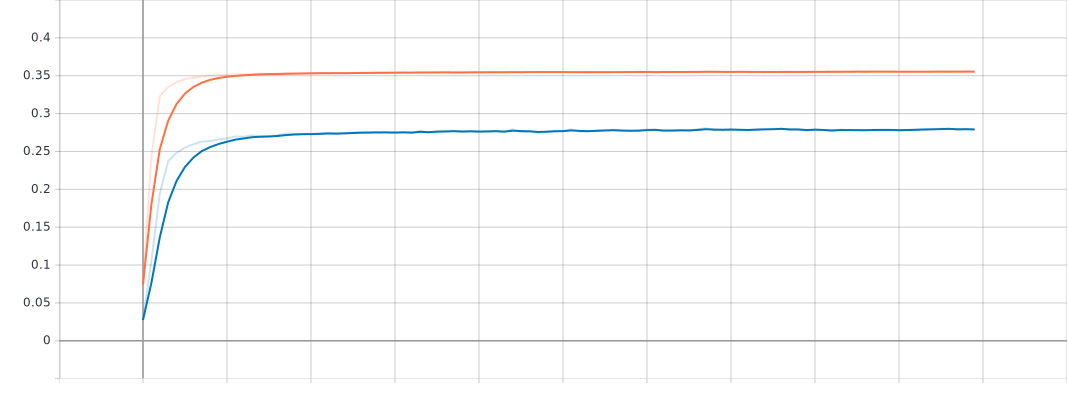
\includegraphics[width=0.45\textwidth]{../../References/medium/accuracy.png}
                \label{fig:accuracy}
            }
            \hfill
            \subfigure[Loss]{
                \centering
                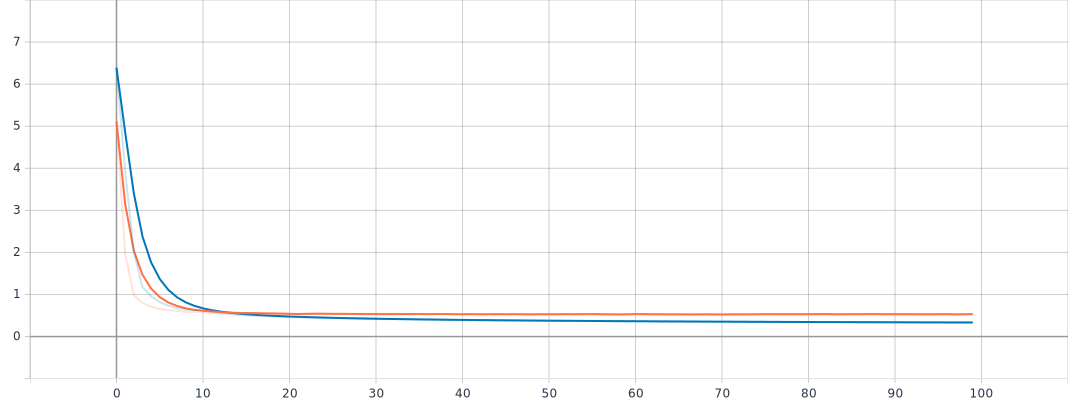
\includegraphics[width=0.45\textwidth]{../../References/medium/loss.png}
                \label{fig:loss}
            }
            \caption{Metrics for the medium data set}
            \label{fig:metrics}
        \end{figure}
        
        The model was trained 100 epochs on the (small and) medium data set, at each one testing and measuring accuracy (see Figure \ref{fig:accuracy}) and loss (see Figure \ref{fig:loss}). In the end, the results were validated using a validation set of 1518 pairs of sentences. From the graphs, it can be seen how these values converge, and also, the loss tends to zero. The model implemented in the presented work obtained a competitive BLEU score of 20.56 for text corrections in Romanian with a modest training set. With an increased training set, it got a score of 33.29, as shown in Table \ref{tab:training-results}, representing a substantial improvement.
        
        \begin{table}[h]
            \caption{Training results}
            \label{tab:training-results}
            \centering
            \begin{tabular}{|c|c|c|c|}
                \hline
                Data set & Epochs & BLEU Score & Training time     \\
                \hline
                Small    & 100    & 20.56      & 9.66 sec. / epoch \\
                \hline
                Medium   & 100    & 33.29      & 99 sec. / epoch   \\
                \hline
                Large    & 5      & 45.29      & 1032 sec. / epoch \\
                \hline
            \end{tabular}
        \end{table}
        
    \section{Interpretation of the Results}
        
        In Figure \ref{fig:attention-examples}, some examples of running the model on different input sentences are presented. Attention was measured at the output (second substrate) of the last decoder layer of the decoder. The examples presented in the figure \vpageref[above]{fig:attention-examples} are also fully corrected cases \ref{fig:2}, partially corrected sentences \ref{fig:5}, and also sentences with errors or that could not be corrected \ref{fig:3}.
        
        \begin{figure}[htbp]
            \centering
            \subfigure[BLEU score: 1.0000]{
                \centering
                \includegraphics[width=0.45\textwidth]{../../References/medium/2.png}
                \label{fig:2}
            }
            \hfill
            \subfigure[BLEU score: 0.7071]{
                \centering
                \includegraphics[width=0.45\textwidth]{../../References/medium/5.png}
                \label{fig:5}
            }
            \subfigure[BLEU score: 0.2741]{
                \centering
                \includegraphics[width=0.45\textwidth]{../../References/medium/3.png}
                \label{fig:3}
            }
            \caption{Attention Examples}
            \label{fig:attention-examples}
        \end{figure}
        
    \section{Conclusion}
        
        Compared to the model proposed in "Attention Is All You Need" \cite{vaswani2017attention}, which was trained twelve hours on eight P100 GPUs, the implemented model was prepared on the medium data set for almost three hours and on the large set for an hour and a half (only five epochs). Only one super data set was used for modeling, and no comparisons could be made with other data sets. Unfortunately, the field development did not make it possible to compare the implemented model with other models. Furthermore, this implementation is a starting point in field development. It can be used in the construction and modeling of high-performance competitive technologies for text corrections in Romanian.
        
    \bibliography{bibliography}
    
\end{document}
